\documentclass[12pt, a4paper]{article}

\usepackage[utf8]{inputenc}
\usepackage{color}
\usepackage{graphicx}
\usepackage{multirow}
\usepackage{multicol}
\usepackage{subcaption}
\usepackage{mathtools}
\usepackage{authblk}
\usepackage[left=1.2in,right=1.2in,top=1.5in,bottom=1in]{geometry}

\title{CSE 300: Online Assignment}

\author{Md Shamsuzzoha Bayzid}
\author{Mahjabin Nahar}
\author{Md Shariful Islam Bhuyan}
\author{Md Saidur Rahman}

\affil[]{}

\date{June, 2021}


\begin{document}
	
\maketitle

\section{Introduction}
	This assignment has been designed to assess the preparation of the students
	in writing scientific articles using \LaTeX. This assignment covers a variety of
	components that are commonly used in scientific manuscripts
	
\subsection{Equations}
	Let $C$ be a simple piecewise smooth curve that bounds a region $D$ in the
	plane. If $P(x, y)$ and $Q(x, y)$ have continuous partials in an open region
	containing $D$, then \\
	$\int_C P dx + Q dy = \iint_D \frac{\partial Q}{\partial x} - \frac{\partial P}{\partial y} dA$
	
	If \textbf{F} is a vector field with third component 0 defined on a domain $D$
	enclosed by boundary $C$ then \\
	$\oint_C \textbf{F} \cdot d\textbf{r} = \iint_D(\nabla \times \textbf{F}) \cdot \textbf{k}dA$
	
	Similarly, if $C$ is defined by $\textbf{r}(t) = \langle x(t),y(t) \rangle$ \\
	$\oint_C \textbf{F} \cdot \textbf{n} ds = \iint_D \nabla \cdot \textbf{F}dA$
	
\subsection{Tables}
	We wish to place the Table at the bottom of the page.
	
\subsection{Figures}
	We intend to put Figure \ref{fig:1} at the top of a page.

\pagebreak
	
\section{Conclusions}
	The major objectives of this assignment are listed below (please do not ignore
the font sizes).

	\begin{itemize}
		\item\LARGE To assess the ability of the students in preparing
		manuscripts in \LaTeX.
		\item\Large To see if the students have adequately practiced different
		aspects of writing in \LaTeX.
		\item\large To see if the students can add various basic components (e.g., tables, figures, equations) to a \LaTeX manuscript.
		\item\normalsize To see if the students can leverage the available materials (both offline and online) to do something which has not explicitly been taught in the class.
	\end{itemize}

\pagebreak

	\begin{table}
	\begin{tabular}{|l||l|l|l|}
		\hline 
		
		\multicolumn{4}{|c|}{Item List} \\
		\hline 
		
		Item Name or &
		ALPHA 2 Code &
		ALPHA 3 Code &
		Numeric Code \\
		
		Product Name & & & \\
		\hline 
		
		\multirow{2}{*}{Item001}  &
		\multirow{2}{*}{AF}  &
		\multirow{2}{*}{AFG}  &
		001 \\
		
		\multirow{2}{*}{}  &
		\multirow{2}{*}{}  &
		\multirow{2}{*}{}  &
		002 \\
		\hline 
		
		Item002 & 
		AX &
		ALA & 
		003 \\ 
		\hline 
		

		\multirow{4}{*}{Item003}  &
		\multirow{4}{*}{AL}  &
		\multirow{4}{*}{ALB}  &
		004 \\
		
		\multirow{4}{*}{}  &
		\multirow{4}{*}{}  &
		\multirow{4}{*}{}  &
		005 \\
		
		\multirow{4}{*}{}  &
		\multirow{4}{*}{}  &
		\multirow{4}{*}{}  &
		006 \\
		
		\multirow{4}{*}{}  &
		\multirow{4}{*}{}  &
		\multirow{4}{*}{}  &
		008 \\
		\hline
		
		\multirow{2}{*}{Item004}  &
		\multirow{2}{*}{DZ}  &
		\multirow{2}{*}{DZA}  &
		009 \\
		
		\multirow{2}{*}{}  &
		\multirow{2}{*}{}  &
		\multirow{2}{*}{}  &
		010 \\
		\hline 
		
		\multirow{2}{*}{Item005}  &
		\multirow{2}{*}{AS}  &
		\multirow{2}{*}{ASM}  &
		011 \\
		
		\multirow{2}{*}{}  &
		\multirow{2}{*}{}  &
		\multirow{2}{*}{}  &
		012 \\
		\hline 
		
		Item006 & 
		AD &
		AND & 
		013 \\ 
		\hline 
		
		Item007 & 
		AO &
		AGO & 
		014 \\ 
		\hline 
		\hline 
		
	\end{tabular}
	\end{table}

\pagebreak

	\begin{figure}[t]
		\centering
		\begin{subfigure}{0.8\textwidth}
			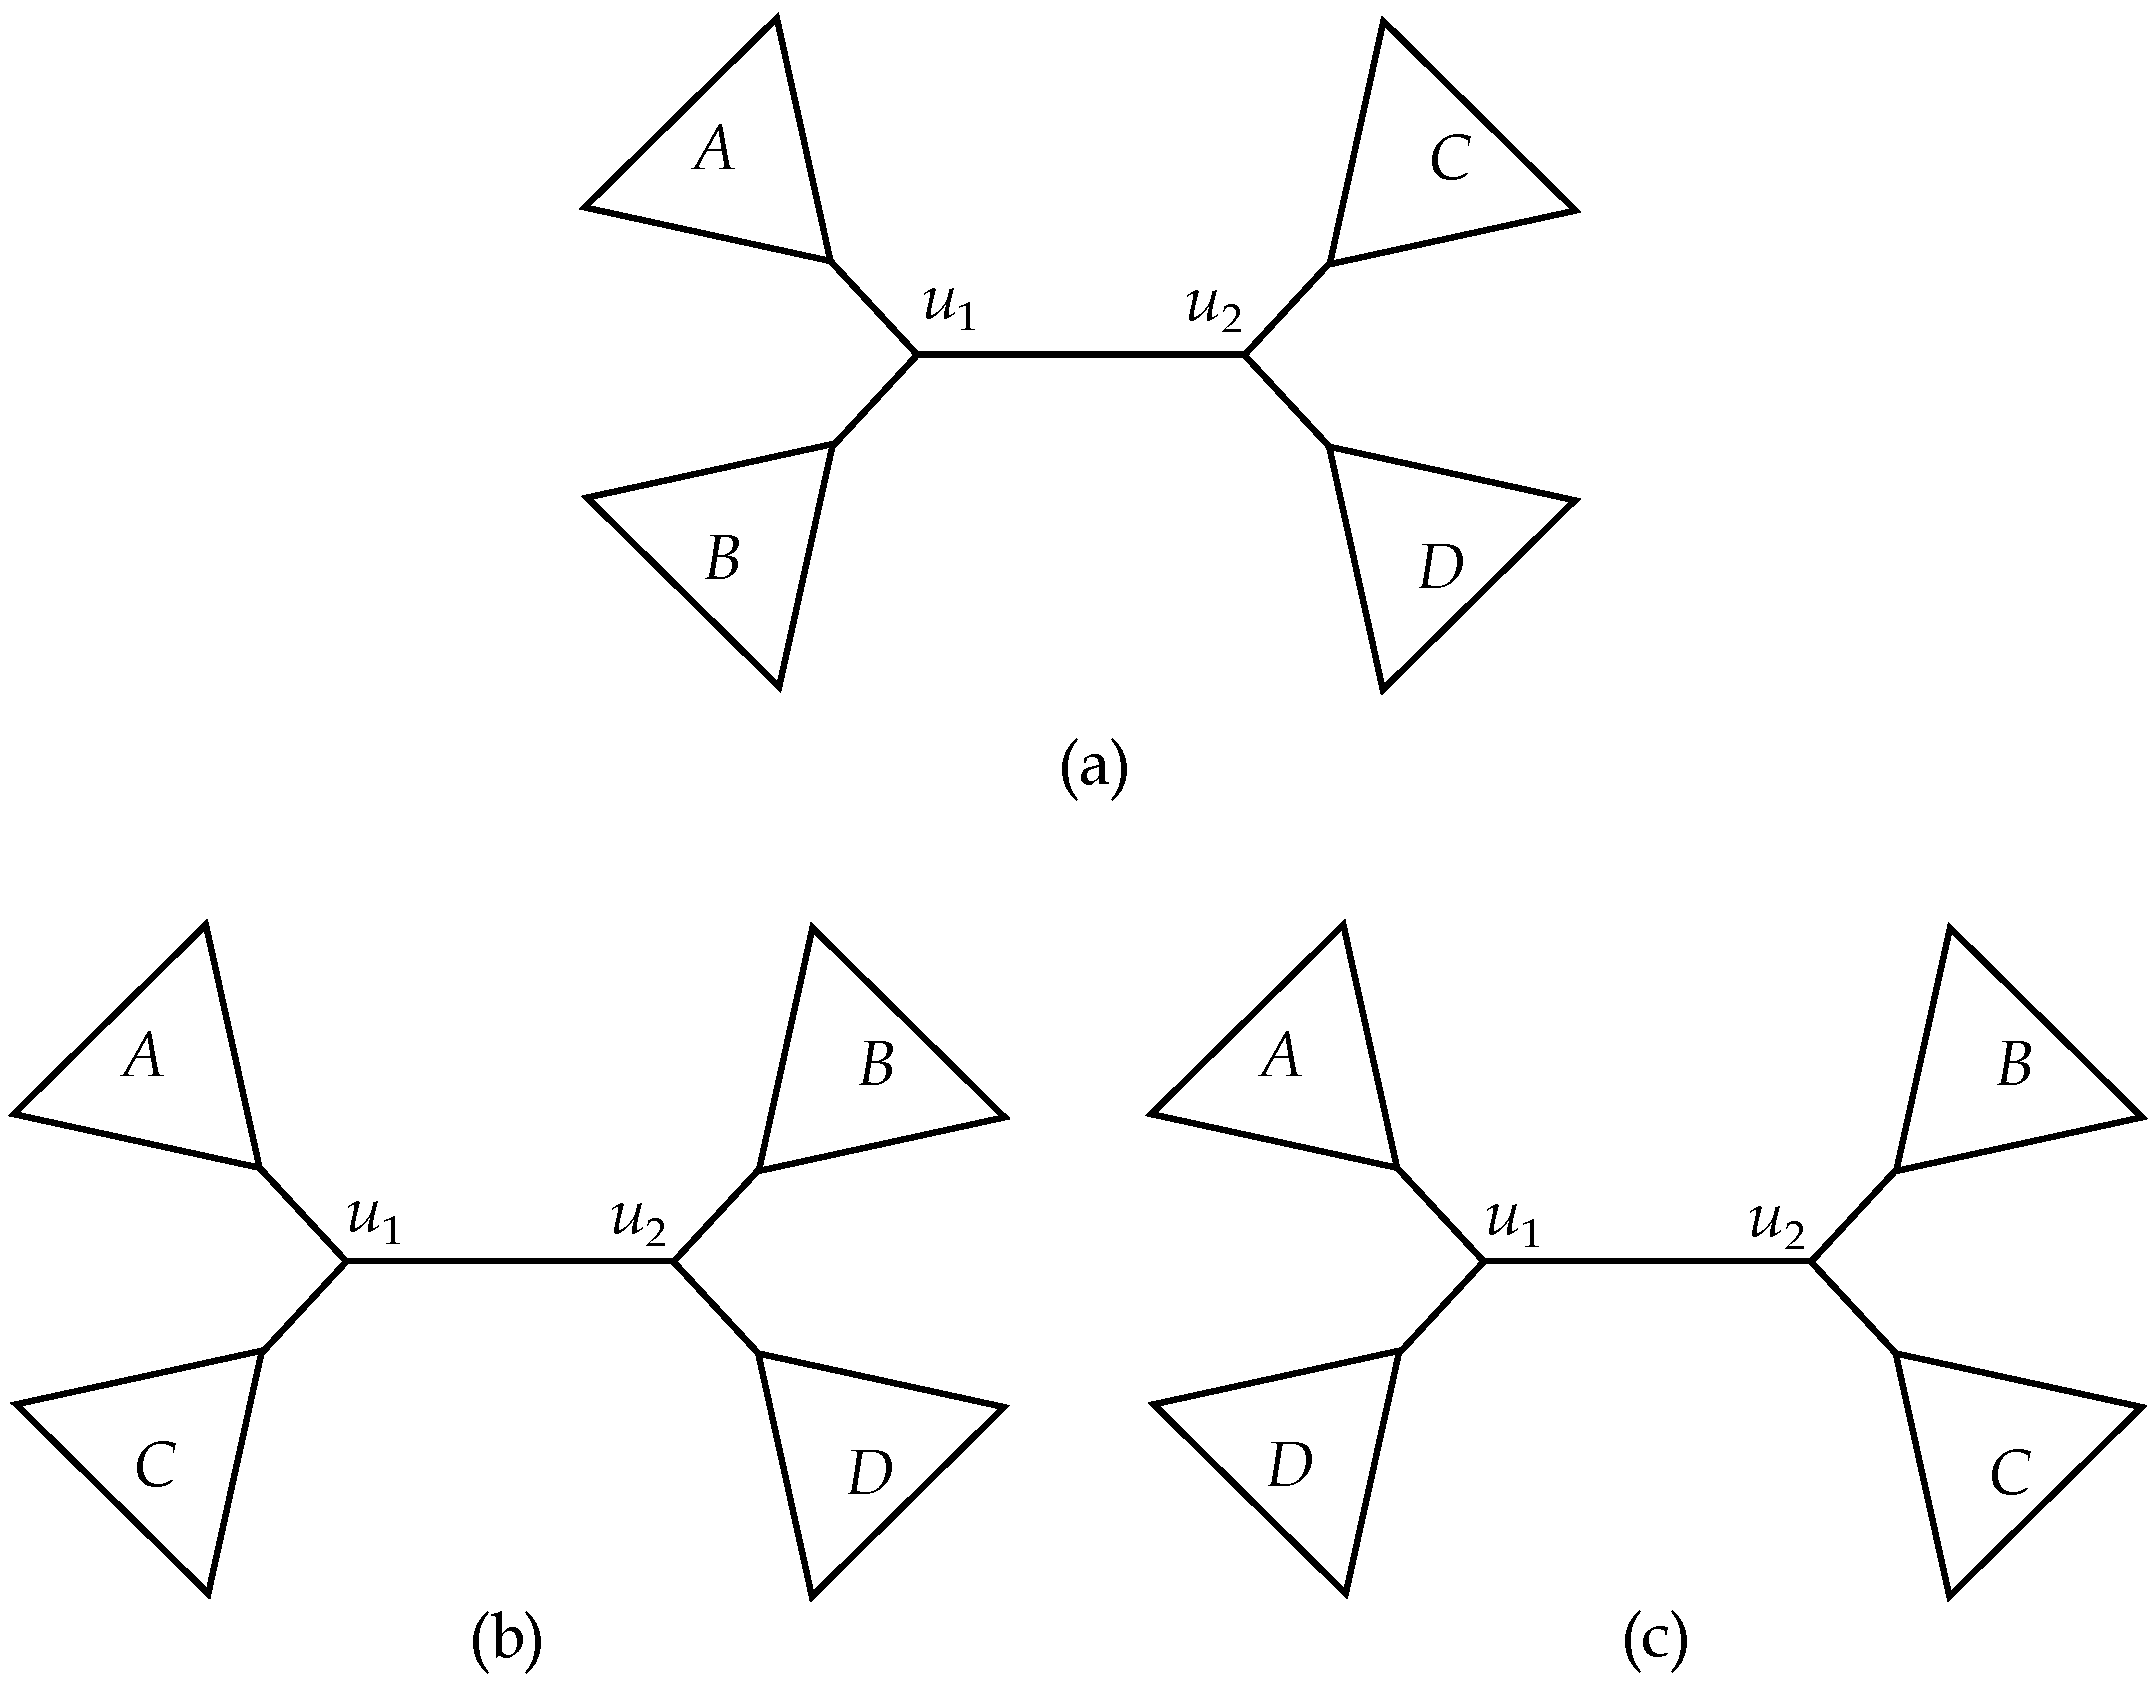
\includegraphics[width=\textwidth,angle=180]{Figure3}
		\end{subfigure}
		\hfill
		
		\begin{subfigure}{0.8\textwidth}
			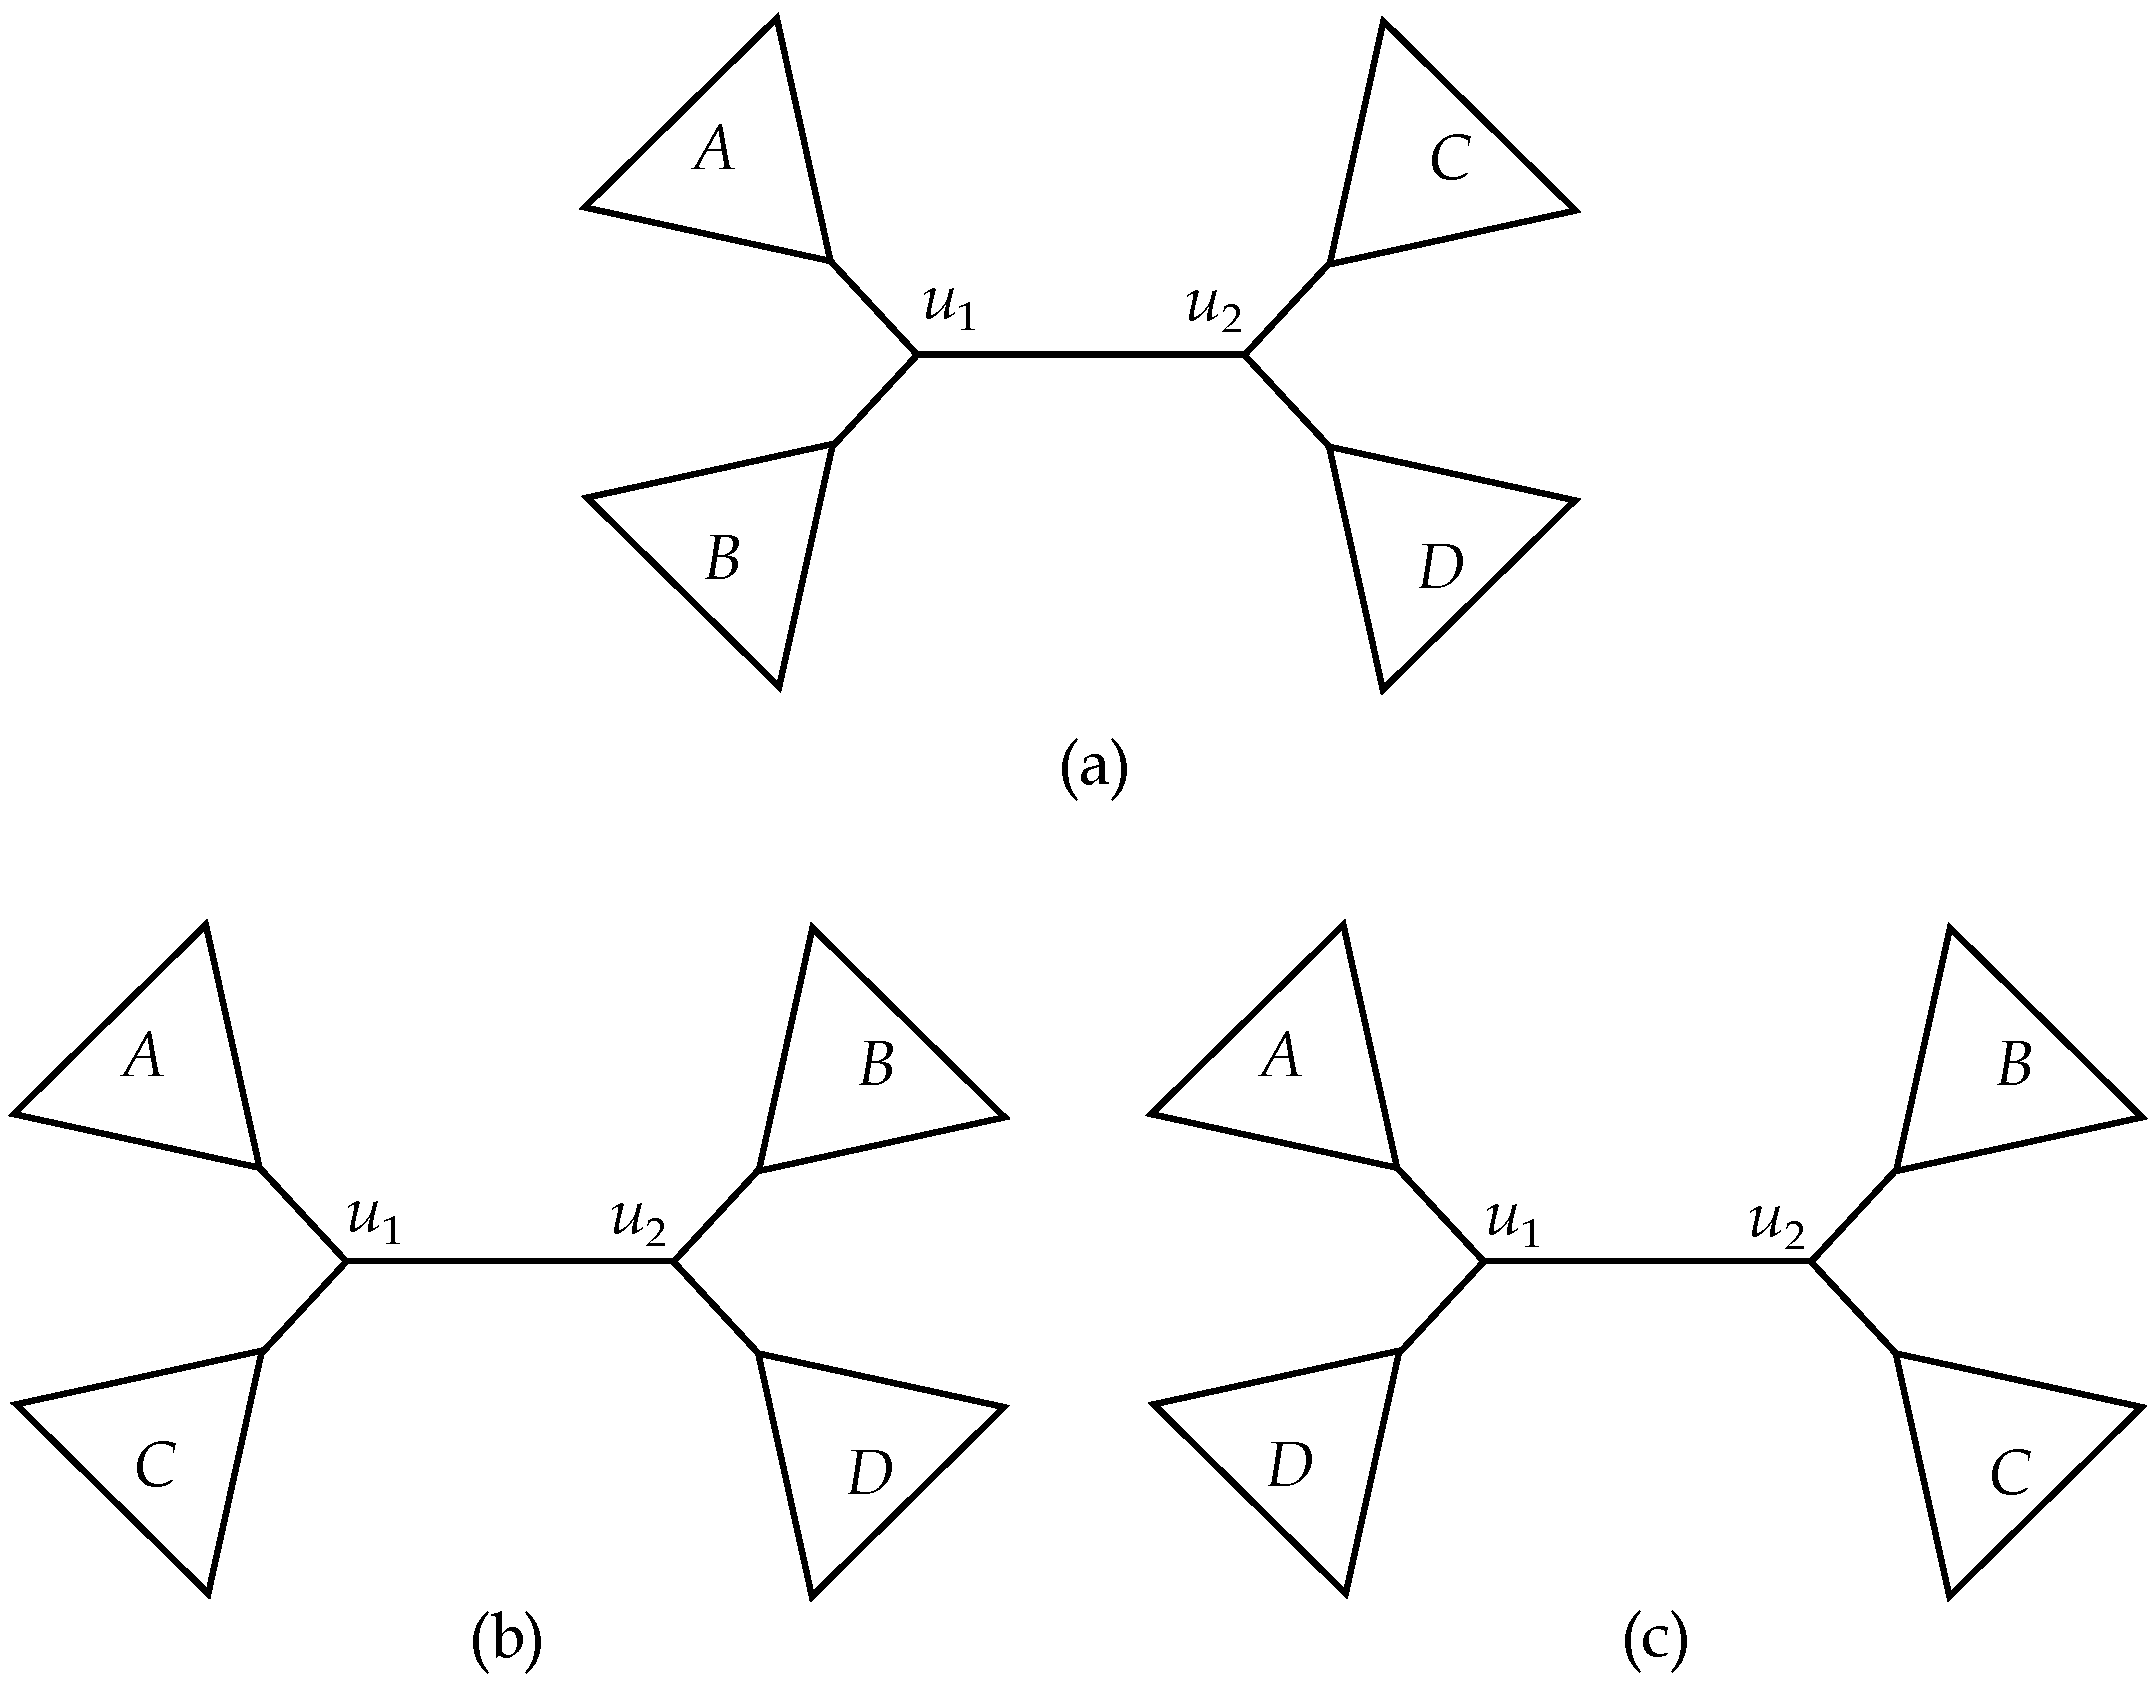
\includegraphics[width=\textwidth]{Figure3}
		\end{subfigure}
		
		\caption{\textbf{Same figure upside down}}
		\label{fig:1}
	\end{figure}

\end{document}